\chapter{Methodology}
\label{chap:met}
This chapter presents the formal basis required to understand the implementation part. Section \ref{met:phicalc} briefly describes the relevant parts of $\varphi$-calculus: its syntax and semantics. Section \ref{met:eo} explains how $\varphi$-calculus maps to EO, the intermediate representation the analyzers operate on. Section \ref{met:encoding} shows how to encode basic object-oriented constructs (classes, methods, inheritance) by means of EO. Sections \ref{met:mutualrec} and \ref{met:unjustified} explain their respective defect type and how it can be detected in an EO program.

\section{$\varphi$-calculus}
\label{met:phicalc}

EO is a programming language that implements $\varphi$-calculus, a formal model for object-oriented programming languages initially introduced by Bugayenko \cite{eolang}. In this thesis we use a refinement of $\varphi$-calculus proposed by Kudasov and Sim \cite{kudasov}.

\subsection{Objects and attributes}
At the heart of $\varphi$-calculus lies the concept of \textbf{object}.

\begin{definition}[Objects and attributes]
    An \textbf{object} is a set of pairs $\mkObject{n_0 \mapsto o_0, n_1 \mapsto o_1, \hdots, n_i \mapsto o_i, \hdots}$, where $n_i$ is a unique identifier and $o_i$ is an object. Such pairs are known as \textbf{attributes}. The first element is the \textbf{attribute name} the second element is the \textbf{attribute value}. An empty set $\mkObject{}$ is also a valid object. An attribute where the second element is $\mkObject{}$ is called \textbf{void} or \textbf{free}. Otherwise, it is known as \textbf{attached}.
\end{definition}

Attributes of object can be accessed by their names via the dot notation:
\begin{align*}
    \mkObject{x \mapsto y}.x \rightsquigarrow y
\end{align*}
In this case, this would reduce to just object $y$, which is defined elsewhere. $\rightsquigarrow$ means "is reduced to" or "evaluates to".

\subsection{Application}
Application can be used to create a new object where the values of the some or all free attributes are set. In other words, application can be used to create \textit{closed} objects from \textit{abstract} objects.

\begin{definition}[Abstract and closed objects]
    If an object has one or more free attributes it is called \textbf{abstract} or \textbf{open}. Otherwise, it is called \textbf{closed}.
\end{definition}

For example, object $a$ in \ref{met:app} corresponds to a point in a two-dimensional space with coordinates $x = 1$, $y = 2$. The objects $1$ and $2$ can be defined in terms of $\varphi$-calculus, however the definition itself is out of the scope of this thesis.

\begin{align}
    point := \mkObject{x \mapsto \mkObject{}, y \mapsto \mkObject} \\
    \label{met:app}
    a := point(x \mapsto 1, y \mapsto 2)                           \\
    a \rightsquigarrow \mkObject{x \mapsto 1, y \mapsto 2}
\end{align}


\subsection{Locators}

The revisision of $\varphi$-calculus by Kudasov and Sim \cite{kudasov} also defines special objects called \textbf{locators}, which are denoted as $\rho^i$, where $i \in \mathbb{N}$. Locators allow objects to reference other objects relatively to the object where the locator is used. For example, this can be used to (but is not limited to) encode definition of attributes in terms of other attributes of this object. Suppose there is an object $x$:
\begin{align*}
    x := \mkObject{a \mapsto \rho^0.b, b \mapsto c}
\end{align*}
The expression $x.a$ would be reduced to the value of object $c$. This happens because $x.a$ references $x.b$ via $\rho^0$, which means the immediate enclosing object. In more complicated examples, like \ref{met:complex}.

\begin{align}
    \label{met:complex}
    x := \mkObject{a \mapsto \mkObject{c \mapsto \rho^1.b}, b \mapsto d} \\
    x.a.c \rightsquigarrow d
\end{align}

$\rho$ can be used to define attributes of inner objects in terms of attributes of outer objects, or even outer objects themselves.

\subsection{$\varphi$-attribute}
Objects can define a special attribute with name $\varphi$. This attribute redirects attribute access to its value when the enclosing object does not have an attribute with such a name (fig. \ref{met:phi}).

\begin{align}
    \label{met:phi}
    a := \mkObject{d \mapsto y}                    \\
    \label{met:decorated}
    x := \mkObject{\varphi \mapsto a, c \mapsto g} \\
    x.d \rightsquigarrow x.\varphi.d \rightsquigarrow y
\end{align}

If the attribute is present both in the object and its $\varphi$-attribute, the attribute in the object takes precedence:
\begin{align*}
    a := \mkObject{d \mapsto y}                             \\
    x := \mkObject{\varphi \mapsto a, \textbf{d} \mapsto g} \\
    x.d \rightsquigarrow g
\end{align*}

In \ref{met:decorated}, Bugayenko \cite{eolang} refers to object $a$ as \textbf{decorated object}, where the "decorated" part refers to the decorator pattern described in \cite[Chapter 4]{GOFPatterns}. This technique of extending an object is also known as \textit{delegation} \cite{raiha_delegation:_1994} in object-oriented languages.

\subsection{Complete example}
Tying everything together, figure \ref{fig:fibo} shows how $\varphi$-calculus can be used to compute Fibonacci numbers.

% fib ->
%   [ n -> ?
%   , @ -> n.less(_1 -> 2).if(
%       _1 -> n
%     )(
%       _2 -> fib(n -> n.sub(_1 -> 1)).add(_1 -> fib(n -> n.sub(_1 -> 2)))
%     )
%   ]
% ].fib(n -> 7)
\begin{figure}
    \begin{align*}
        fib := &\mkObject{                                    \\
            n &\mapsto \mkObject{},                           \\
            \varphi &\mapsto \rho^0.n.less(n \mapsto 2).if( \\
            &ifTrue \mapsto n,                                \\
            &ifFalse \mapsto                                  \\
            &fib(n \mapsto \rho^0.n.sub(n \mapsto 1))\\
            &.add(n \mapsto fib(n \mapsto \rho^0.n.sub(n \mapsto2)\\)\\)\\)\\
        }
    \end{align*}
    \caption{Fibonacci numbers in $\varphi$-calculus}
    \label{fig:fibo}
\end{figure}

% \subsection{Dataization}
% $\varphi$-attribute plays an important role in the process of \textit{dataization}, which is a term coined by Bugayenko in \cite{eolang} that describes the evaluation of an EO program.

\section{EO}
\label{met:eo}
EOLANG, or simply EO, is a programming language created by Bugayenko \cite{eolang} which is a direct implementation of $\varphi$-calculus with some extensions. However, their implementation contains features that are irrelevant to the scope of this thesis. Moreover, there is a notable difference between Bugayenko version of EO and $\phi$-calculus by \cite{kudasov} in the definition of locators (or "parent objects"). In the work by Bugayenko locators are \textit{attributes}, whereas in \cite{kudasov} they are \textit{objects}. Consequently, in this thesis, similarly to the $\varphi$-calculus, we are going to use a different version of EO which is a direct translation of the calculus defined in \ref{met:phicalc}. The table of translation is shown in figure \ref{fig:phitoeo}.

\begin{figure}
    \begin{center}
        \begin{tabular}{|c|c|c|}
            \hline
                                & $\varphi$-calculus         & EO \\
            \hline
            Objects             & $obj := \mkObject{a \mapsto x, b \mapsto y}$ &  \lstinputlisting{code/objects.eo}\\
            \hline
            Free Attrubutes     &   $point := \mkObject{x \mapsto \mkObject{}, y \mapsto \mkObject}$   &  \lstinputlisting{code/free_attributes.eo}   \\
            \hline
            Application &     $a := point(x \mapsto 1, y \mapsto 2)$ & \lstinputlisting{code/application.eo} \\
            \hline
            $\varphi$-attribute & $x := \mkObject{\varphi \mapsto a, c \mapsto g}$ & \lstinputlisting{code/phi_attribute.eo}   \\
            \hline
            Fibonacci example & Fig. \ref{fig:fibo} & \lstinputlisting{code/fibonacci.eo}   \\
            \hline
            $\rho^0$ & $\rho^0$ &  \$ \\
            \hline
            $\rho^1$ & $\rho^1$ &  \textasciicircum \\
            \hline
            $\rho^3$ & $\rho^3$ &  \textasciicircum.\textasciicircum.\textasciicircum \\
            \hline
        \end{tabular}
    \end{center}
    \caption{Mapping $\varphi$-calculus to EO}
    \label{fig:phitoeo}
\end{figure}

\section{Describing object-oriented programs with EO}
\label{met:encoding}
Before analyzing programs written in object-oriented programming languages, it is necessary to translate them into EO while preserving the semantics of the original language. This chapter presents a simplified version of such an encoding that is assumed by analyzers described in this thesis.

\subsection{Classes}
Classes are modelled as closed EO objects. Class-level (i.e. "static") attributes become attributes of the class object. Constructor is represented by an attribute-object "new" of the class object. This object may take parameters to produce an instance of the object.

All instance attributes and methods are defined inside the object returned by the "new" object. Inheritance is modelled as decoration in EO. So, a full example of EO translation would look like this. Class instances (a.k.a objects in Java) are created
by applying the "new" object to the required parameters.

\subsection{Methods}
Methods are modelled as EO objects, similarly to classes. These objects can take parameters.
Instance methods are required to accept a special \textbf{self} attribute in addition to other parameters. This parameter is used to pass an instance of the object calling the method (hence the name - "self").
"self" parameter can be used to call instance methods inside other instance methods.

The return value of the method is represented by the value of the $\varphi$ attribute ("@" symbol in EO). In order to call the instance method we need to instantiate the object first. Then we can call the method by accessing the instance's attribute with the method name and passing the instance object to it as the first argument.

\section{Detecting Unanticipated Mutual Recursion}
\label{met:mutualrec}
\subsection{Problem Statement}
Unanticipated mutual recursion is a problem that occurs as a result of unconstrained inheritance. Suppose we have an object named Base with two methods - $f$ and $g$. Method $g$ calls method $f$, whereas $f$ does not.


Then, there is a class called Derived that extends Base and redefines the method $f$ in a way that it calls $g$. When we call a method $f$ on an instance of Derived, we get a stack overflow error: method $f$ calls method $g$, method $g$ calls method $f$ and so on (figure \ref{fig:mutualrec_basic}).

It is important to note that we are not interested in detecting mutual recursion between the two methods of the same class. We are only interested the cases where mutual recursion occurs as a result of redefining one of the methods of the superclass. The example in fig. \ref{fig:oddeven} shows the class with two mutually-recursive methods "isOdd" and "isEven". In this case the recursion is anticipated and necessary, so it is not a defect.

\begin{figure}
    \centering
    \begin{subfigure}{0.4\textwidth}
        \lstinputlisting[language=Java]{code/mutualrec.java}
        \caption{Java}
    \end{subfigure}
    \hfill
    \begin{subfigure}{0.4\textwidth}
        \lstinputlisting{code/mutualrec.eo}
        \caption{EO}
    \end{subfigure}
    \caption{Example of unanticipated mutual recursion}
    \label{fig:mutualrec_basic}
\end{figure}

\begin{figure}
    \centering
    \begin{subfigure}{0.4\textwidth}
        \lstinputlisting[language=Java]{code/NumericOps.java}
        \caption{Java}
    \end{subfigure}
    \hfill
    \begin{subfigure}{0.4\textwidth}
        \lstinputlisting{code/numeric_ops.eo}
        \caption{EO}
    \end{subfigure}
    \caption{Example without unanticipated mutual recursion.}
    \label{fig:oddeven}
\end{figure}

\subsection{Proposed solution}
The solution to the problem lies in detecting the cycles in the call-graphs of all the objects. For each class-object in the program, do the following:
\begin{enumerate}
    \item Detect the decorated class-object, all methods, and for each method in the class detect all the methods it calls. If the method that is called exists in the class-object, mark it as \textit{resolved}. Otherwise, mark it as \textit{partially-resolved}. The set of mappings between the methods of the class and the methods that each of the methods calls is considered a \textit{partial call-graph} of the object.
    \item After that the tree is traversed again to convert all the partially-resolved calls to fully resolved calls. To do that we need to calculate the \textit{complete call-graph} of the object, which contains the methods from the object itself, as well as the methods from the decorated object. This is done by \textit{extending} the partial call-graph of the decorated object with the partial call-graph of the decorating objects. Hereinafter we use the terms \textbf{child} and \textbf{parent} to refer to the decorating object and the decorated object respectively. The extension procedure is defined as follows: 
    \begin{enumerate}
        \item if the method is present in the parent call-graph, but is absent in the child call-graph, it is left as is. 
        \item if the method is present in the child call-graph but does not exist in the parent call-graph, it is added to the parent call-graph.
        \item if the method is present both in the child call-graph and the parent call-graph, all the occurrences of the method in the parent call-graph are replaced by the child's version of the method.
    \end{enumerate} 
    \item After the object's call-graph is resolved, perform the depth-first search \cite{dfs} to find the cycles in the complete call-graph. After all the cycles are found, exclude the cycles that contain only the methods from the same object. 
\end{enumerate}

\section{Detecting Unjustified Assumption in Subclass}
\subsection{Problem Statement}
\label{met:unjustified}
This defect \cite[Section 3.3]{fragilebaseclass} occurs when the superclass is refactored by \textit{inlining} the calls to the method that can be redefined by the subclass. The term inlining refers to replacing the method call with its body. Consider an example \pic{fig:unjustified_before}. Class $M$ extends class $C$, redefining method $l$ to weaken its precondition. Consequently, the precondition in method $m$ of class $M$ is also weakened, because it relies on calling the method $l$. 

Now, suppose that class $C$ comes from some external library, and class $M$ is defined in the user code. Library maintainer decides to refactor class $C$ by inlining the call to $l$ in method $m$ \pic{fig:unjustified_after}. Observe what happens to the class $M$. Now that $m$ in class base has an assert, the redefinition of method $n$ in class $M$ has its precondition strengthened as compared to its version in class $C$. Therefore, the seemingly safe refactoring in base class broke the invariants in the subclasses. The name of the defect come from the fact that the subclasses usually $M$ \textit{assume} that the method $m$ should be implemented in terms of method $l$. The examples in fig. \ref{fig:unjustified_before} and \ref{fig:unjustified_after} show that such an assumption is indeed not justified, and the maintainers of class $C$ can change it as they deem fit.

\begin{figure}
    \centering
    \begin{subfigure}{0.4\textwidth}
        \lstinputlisting[language=Java]{code/Unjustified.java}
        \caption{Java}
    \end{subfigure}
    \hfill
    \begin{subfigure}{0.4\textwidth}
        \lstinputlisting{code/unjustified.eo}
        \caption{EO}
    \end{subfigure}
    \caption{Example of unjustified assumption in subclass (before revision)}
    \label{fig:unjustified_before}
\end{figure}

\begin{figure}
    \centering
    \begin{subfigure}{0.4\textwidth}
        \lstinputlisting[language=Java]{code/UnjustifiedRevised.java}
        \caption{Java}
    \end{subfigure}
    \hfill
    \begin{subfigure}{0.4\textwidth}
        \lstinputlisting{code/unjustified_revised.eo}
        \caption{EO}
    \end{subfigure}
    \caption{Example of unjustified assumption in subclass (after revision)}
    \label{fig:unjustified_after}
\end{figure}

\subsection{Proposed Solution}
We propose the following approach for detecting the methods where inlining of the calls may lead to breaking changes in subclasses:
\begin{enumerate}
    \item An \textit{initial} representation of the program is produced. This representation is a tree-like data structure which preserves the nesting relations between objects. So, the objects which contain other objects are the roots of their respective subtrees, whereas the container objects are the subtrees or leaves.
    \item We produce a \textit{revision} of the initial program representation where all the calls to the methods are inlined. 
    \item In both versions, for each of the class-objects, for each method in the class-object, a set of \textit{properties} is inferred.  These properties can be thought of as an implicit contract \cite{meyer} of each method. In addition to the implicit properties, the explicit properties which come in the form of \textit{assert} statements in the source code are also taken into account. In order to infer the properties of the method, partial interpretation of its body is performed. The interpretation is limited to basic numeric operations, numeric and boolean values and method calls. The inference rules are described in greater detail in fig. \ref{fig:props}.
    \item After all the properties are inferred, the following predicate should hold true for both the initial and the revised versions:
    \begin{align*}
        P_{init} \implies P_{rev}
    \end{align*}
    If it doesn't hold for some class-object, it means that the revision of one of its superclasses introduces a breaking change, which weakens the precondition of some its methods. 
\end{enumerate}

\begin{figure}
    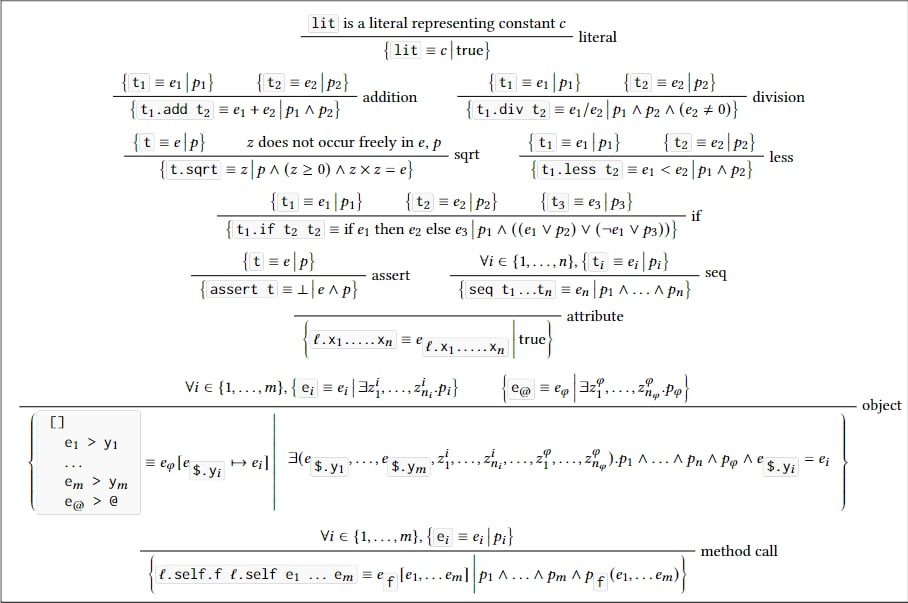
\includegraphics[width=\textwidth]{figs/properties}
    \caption{Rules for property inference in detection of unjustified assumption in subclass.}
    \label{fig:props}
\end{figure}

